
\documentclass[trackchanges,twocolumn]{aastex631}
\usepackage{amssymb}
\usepackage{float} \usepackage{listings}
\usepackage{xcolor}
\usepackage{amsmath}


\begin{document}
\makeatletter
\let\frontmatter@title@above=\relax
\makeatother

%Define Commands
\newcommand\lsim{\mathrel{\rlap{\lower4pt\hbox{\hskip1pt$\sim$}}
\raise1pt\hbox{$<$}}}
\newcommand\gsim{\mathrel{\rlap{\lower4pt\hbox{\hskip1pt$\sim$}}
\raise1pt\hbox{$>$}}}
\newcommand{\CS}[1]{{\color{red} CS: #1}}

% Evidence against a binary origin for long secondary periods from Gaia astrometry
\title{\Large Gaia astrometry disfavors a binary origin for long secondary periods}

\shorttitle{Evidence against a binary origin for LSPs}
\shortauthors{Shariat, El-Badry, \& MacLeod}

\author[0000-0003-1247-9349]{Cheyanne Shariat}
\affiliation{Department of Astronomy, California Institute of Technology, 1200 East California Boulevard, Pasadena, CA 91125, USA}

\author[0000-0002-6871-1752]{Kareem El-Badry}
\affiliation{Department of Astronomy, California Institute of Technology, 1200 East California Boulevard, Pasadena, CA 91125, USA}

\author[0000-0002-1417-8024]{Morgan MacLeod}
\affiliation{Institute for Theory \& Computation, Center for Astrophysics, Harvard \& Smithsonian, Cambridge, MA 02138, USA}

\correspondingauthor{Cheyanne Shariat}
\email{cshariat@caltech.edu}

\begin{abstract}
Approximately one-third of luminous pulsating red giant stars exhibit long secondary periods (LSPs): stable photometric variability with periods of several months to years in addition to their much shorter primary pulsation cycles.
Now nearly a century after their discovery, the physical origin of LSPs remains unresolved. A leading explanation invokes binarity, in which the LSP corresponds to the orbital period of a low-mass companion responsible for both the photometric variability and the radial-velocity (RV) modulation. We test this hypothesis using a nearby sample of LSP stars from the {\it Gaia} Focused Product Release, which provides multi-epoch RVs and contemporaneous optical photometry. We find that interpreting the observed RV variability as orbital motion implies companion masses narrowly distributed around $M_2 \approx 0.1~{\rm M_\odot}$ with separations of 1--3 au, placing them squarely in the brown dwarf desert observed around their solar-type progenitors.
Assuming such companions exist, we then forward-model the astrometric signature expected in {\it Gaia} DR3 and predict systematically elevated {\tt RUWE} values for nearby LSPs. In contrast, the observed {\tt RUWE} of nearby LSP stars is systematically lower than these predictions and consistent with most systems exhibiting LSPs being single. This discrepancy rules out low-mass stellar or substellar companions as the dominant origin of LSPs in evolved stars, motivating a further exploration of alternative stellar mechanisms.
\end{abstract}

\section{Introduction}\label{sec:introduction}


Roughly one in three pulsating red giants show photometric variability on timescales of hundreds to thousands of days, in addition to their dominant pulsation periods of tens to hundreds of days \citep[e.g.,][]{Wood99,Wood04, Soszynski04,Soszynski07,Fraser08,Nicholls09,Pawlak21,Pawlak24}.  
These long secondary periods (LSPs) define a distinct sequence in the period--luminosity ($P$-$L$) diagram \citep[sequence~D;][]{Wood99}.
LSPs have been recognized for nearly a century \citep{OConnell33,PayneGaposchkin54,Houk63}, and although extensive observational and theoretical efforts over this time have characterized many of their empirical properties, their physical origin remains uncertain.

A broad range of mechanisms have been proposed to explain LSPs, including pulsation modes \citep{Wood00,Wood04,Nicholls09,Saio23}, oscillatory convective modes \citep{Saio15,Takayama15,Takayama20,CourtneyBarrer26}, rotational modulation by large convective cells or surface inhomogeneities \citep{Stothers10,Soszynski14}, episodic dust formation and non-spherical mass loss \citep{Wood09,Pawlak21}, and low-mass companions producing orbital modulation and/or dust obscuration \citep{Wood99,Derekas06,Soszynski07,Soszynski21,Goldberg24,Decin25}.

The past few decades of LSP studies revealed a number of well-established empirical properties. LSPs remain coherent over many cycles, their light curves are often asymmetric or non-sinusoidal \citep[e.g.,][]{Soszynski14}, their color and effective-temperature variations are modest \citep{Nicholls09,Takayama20}, their radial-velocity amplitudes are only a few km~s$^{-1}$ \citep{Nicholls09}, and they are associated with enhanced mid-infrared excesses relative to non-LSP giants of similar luminosity \citep{Wood09,Pawlak21}. Any successful LSP model must account for this full set of properties \citep[see][for a comprehensive list]{Goldberg24}.

In recent years, binarity has emerged as a dominant hypothesis for the origin of LSPs. In this class of models, the LSP corresponds to the orbital period of a low-mass companion -- either a brown dwarf or low-mass star -- embedded in the extended atmosphere or wind of the red giant \citep[e.g.,][]{Soszynski21}. Periodic obscuration by dust associated with the companion, or by a trailing dusty wake, are invoked to explain the optical variability, while thermal emission and eclipses of the dusty material are proposed to explain the infrared behavior \citep{Wood09,Soszynski21,Goldberg24,MacLeod25}. Recent empirical support for this binary picture has come from mid-infrared light curves, which show features resembling secondary-minima phased with the LSP, interpreted as eclipses of the dusty structure \citep{Soszynski21}. The binary interpretation has gained further prominence through studies of the nearby supergiant Betelgeuse, whose $\sim2100$~day variability period has been modeled as an LSP caused by a close, low-mass companion \citep[e.g.,][]{Goldberg24,MacLeod25}. This picture is potentially supported by radial-velocity, astrometric, X-ray, ultraviolet, and (perhaps) speckle-imaging constraints on Betelgeuse \citep{Goldberg24,MacLeod25,OGrady25,Goldberg25,Dupree26}.

At the same time, the binary hypothesis faces a major demographic difficulty. Interpreting the observed LSP radial velocities as orbital motion implies companions with masses of roughly $0.05$--$0.15~{\rm M_\odot}$ on separations of order $1$--$3$~au \citep[e.g.,][]{Nicholls09}. This is the regime of the brown dwarf desert, a well-established dearth of companions at these masses and separations around solar-type main-sequence stars, the progenitors of most LSP hosts \citep[e.g.,][]{Marcy00,Grether06}. Reconciling this desert with the high incidence of LSPs, $\sim30\%$ of pulsating red giants \citep{Pawlak21}, is a central challenge for binary-based models. 

In addition, Keplerian fits to LSP radial-velocity curves yield a non-uniform distribution of the argument of periastron ($\omega$), which preferentially clusters at $\omega > 180^\circ$ \citep[e.g.,][]{Wood04,Nicholls09}. This implies that most often at periastron the red giant is closest to the observer while the lower-mass companion is farther away -- a configuration that is statistically unlikely for randomly oriented binary systems. Recently, \citet{Decin25} proposed that eccentric low-mass companions embedded in dusty environments, combined with time-in-dust selection effects, may reproduce the observed phase relations and periastron distribution. However, this interpretation still does not reconcile the discrepancy with the brown dwarf desert.

One proposed resolution for the brown dwarf desert problem is that LSP companions may not have formed at their present masses, but instead began as giant planets that subsequently accreted material from the evolving primary \citep[e.g.,][]{Soszynski21}. However, the LSP phenomenon is observed across multiple stages of red-giant evolution \citep[e.g.,][]{Pawlak21, Pawlak24} rather than being confined to the high mass-loss AGB regime, complicating scenarios that rely on strong dust-driven winds to build up companion masses.

Irrespective of their origin, if low-mass companions are responsible for LSPs, they must induce astrometric reflex motion in nearby systems. The high-precision, space-based astrometry provided by the {\it Gaia} mission offers a direct and independent population-wide test of the binary interpretation for LSPs.

In this work, we present a comprehensive test of the binary hypothesis for LSPs using a large, homogeneous sample of LSP red giants from the {\it Gaia} DR3 Focused Product Release \citep{Gaia_FPR}. The {\it Gaia} catalog contains $\sim$4800 LSPs with precise radial velocity time series -- nearly two orders of magnitude more than available in previous studies \citep[e.g.,][]{Nicholls09}.
By combining multi-epoch RVs with high-quality photometry, we infer the companion masses implied by a Keplerian interpretation of the LSPs. We then use a forward model of {\it Gaia} astrometry for binaries \citep[{\tt gaiamock};][]{ElBadry24} to predict the astrometric signatures expected for such systems and assess whether low-mass companions are present in LSP red giants. 

The remainder of the paper is organized as follows. 
In Section~\ref{sec:methodology} we describe our methodology, including our sample selection and subsequent joint RV+astrometry+photometry analysis. In Section~\ref{sec:results} we present our results and test whether LSPs are consistent with binarity. In Section~\ref{sec:discussion} we discuss the implications of our results for existing models of LSPs, and we summarize our conclusions in Section~\ref{sec:conclusions}.

\section{Methodology}\label{sec:methodology}
\subsection{LSP Sample Selection}\label{subsec:methodology_sample}
Throughout this paper, we analyze two samples of LSP stars. The first sample is drawn from the {\it Gaia} Focused Product Release (FPR) \citep[][]{Gaia_FPR} and provides RVs, photometry, and astrometry for all systems, enabling a direct test of the binary hypothesis. This serves as the primary sample used throughout the paper.
A secondary sample, drawn from ASAS-SN \citep[][]{Pawlak24}, lacks RVs but increases the number of LSPs available to assess trends that are not heavily reliant on RVs.

\subsubsection{{\it Gaia} Focused Product Release}\label{subsubsec:methodology_sample_FPR}

The main sample used in this work is the {\it Gaia} FPR catalog of long-period variables (LPVs) with RV time series. The catalog provides epoch RVs and contemporaneous multi-band photometry (in $G,G_{\rm BP},G_{\rm RP}$) for LPV candidates from {\it Gaia} DR3 \citep{Lebzelter23,Gaia_FPR}. The FPR selection is designed to retain only sources with high-quality, well-sampled RV variability with periods consistent with a photometric period. The details of the {\it Gaia} FPR catalog construction are described in \citet{Gaia_FPR}, and we briefly summarize the LSP selection below.


The {\it Gaia} FPR LPV catalog applies a series of stringent quality cuts on the RV data. The cuts include a (i) brightness requirement of $G_{\rm RVS}<12$~mag, (ii) minimum of $12$ RV visibility periods, and (iii) requirement that the uncertainty on the median RV ($\epsilon_{\rm V_R}$) is small compared to the RV amplitude ($\epsilon_{\rm V_R}<0.175\times{\tt rv\_amplitude\_robust}$). Note that ${\tt rv\_amplitude\_robust}$ is the {\it total} peak-to-peak RV amplitude after outlier removal. Additional filtering removes sources with poorly behaved RV time series, including those with more than one rejected RV epoch, significant linear RV trends, or low RV signal-to-noise. After enforcing that the RV-derived period is the same as at least one photometric period (allowing for both $P$ and $2P$), the final FPR catalog contains $9{,}614$ LPVs, of which $6{,}093$ constitute a top-quality subset with fully consistent RV and photometric variability across all bands \citep{Gaia_FPR}. All LSP systems considered in this work are drawn from this top-quality subset. 

LSP stars were selected from the FPR catalog as sources that satisfy \citep[][]{Lebzelter23,Gaia_FPR}:
\begin{equation}\label{eq:gaia_cut}
    A_{\rm G}<0.35~{\rm mag}~~{\rm and}~~ \frac{A_{\rm G}}{{\rm mag}} < 10^{-7} \times \left( \frac{P_{\rm G}}{{\rm days}}\right)^{2.5},
\end{equation}
where $A_{\rm G}$ is the photometric $G$-band semi-amplitude and $P_{\rm G}$ is the corresponding photometric period. Filtering for low-amplitude, long-period variables effectively excludes the majority of fundamental-mode pulsators \citep[][]{Gaia_FPR}.
For the astrometric analysis in Section \ref{subsec:results_ruwe}, we further restrict the sample to nearby stars ($d \leq 1$~kpc; $N=101$). At larger distances, the astrometric wobble due to low-mass companions at few-au separations will typically be too small to be detected by {\it Gaia} and to inflate the {\tt RUWE} value \citep[][]{Belokurov20, Sullivan25, ElBadry25}.

\subsubsection{ASAS-SN variable stars}
\label{subsec:methodology_asas_sample}

We also consider an independent sample of LSP stars identified from ASAS-SN photometry \citep{Pawlak24}, which only minimally overlaps with the {\it Gaia} FPR sample (8 common stars). These systems do not have epoch RVs, and thus companion masses cannot be derived directly. Instead, we assign simulated companion masses by sampling from the {\it Gaia} LSP distribution, which is narrowly peaked at $M_2\approx0.1~{\rm M_\odot}$ (see Section \ref{subsec:results_rvamps}).

\citet{Pawlak24} selected LSP stars from the ASAS-SN Catalog of Variable Stars \citep{Jayasinghe18, Jayasinghe19} and cross-matched them with {\it Gaia} DR3. They identified LSPs using an empirical period--amplitude criterion designed to isolate stars on ``sequence~D'' \citep[e.g.,][]{Wood99} while avoiding contamination from long-period pulsators and ellipsoidal binaries. For each star, the three strongest periods were identified and a period was classified as an LSP if it satisfied
\begin{equation}\label{eq:asas_selection}
    \frac{A_V}{\rm mag} < 1.6~\log \left( \frac{P_V}{\rm days} \right) - 3.7,
\end{equation}
where $P_V$ is the photometric period in days and $A_V$ is the peak-to-peak $V$-band amplitude. This criterion is calibrated using OGLE Large Magellanic Cloud LPVs and was demonstrated to select stars occupying the classical LSP sequence in the $P$-$L$ diagram \citep{Pawlak24}. An additional magnitude-dependent amplitude cut, $A > 0.036V - 0.458$, was imposed on faint stars to mitigate spurious detections, where ASAS-SN photometric uncertainties increase ($\approx 0.1$~mag at $V=17$~mag).

From the \citet{Pawlak24} LSP catalog ($N=55{,}558$), we choose stars with positive {\it Gaia} parallaxes and $d<1.5$~kpc ($N=1{,}601$). The distance cut is a conservative threshold for resolving astrometric motion induced by low-mass companions in {\it Gaia} DR3 \citep[][]{ElBadry24}; the photocenter of a hypothetical LSP binary at $1.5$~kpc is $a_0\lsim0.2$~mas. To exclude residual main-sequence contaminants, we require an absolute {\it Gaia} $G$-band magnitude $M_G < 1$ ($N=1{,}370$). Finally, to avoid very bright sources that are likely affected by saturation or unreliable ASAS-SN photometry, we impose a cut of $G > 5$, leaving a final sample of $N=1{,}362$ red giant LSPs. 


\subsubsection{Summary of the Sample}

Figure \ref{fig:hr_diagram_lsps} shows the location of the {\it Gaia} and ASAS--SN LSP samples on the dust-corrected {\it Gaia} CMD. 
Extinction corrections are derived using the three-dimensional dust map of \citet{Edenhofer24}, which reconstructs the interstellar dust distribution out to $1.25$~kpc (the volume-limit of the figure) from {\it Gaia} XP spectra.
Most systems are evolved RGB and AGB stars, often near or above the tip of the RGB, consistent with previous findings \citep[e.g.,][]{Pawlak21}. In the $d<1.25$~kpc sample, the two catalogs overlap along the evolved giant branch, but ASAS--SN extends to bluer colors and slightly fainter magnitudes on the earlier RGB whereas the {\it Gaia} FPR sample does not. The plotted samples contain $358$ ASAS--SN LSPs and $165$ {\it Gaia} LSPs, and the clearest mismatch is the blue extension at $(G_{\rm BP}-G_{\rm RP})_0 \lesssim 2.5$, where ASAS--SN contains $33$ systems and the {\it Gaia} FPR contains none.

\begin{figure}
\centering
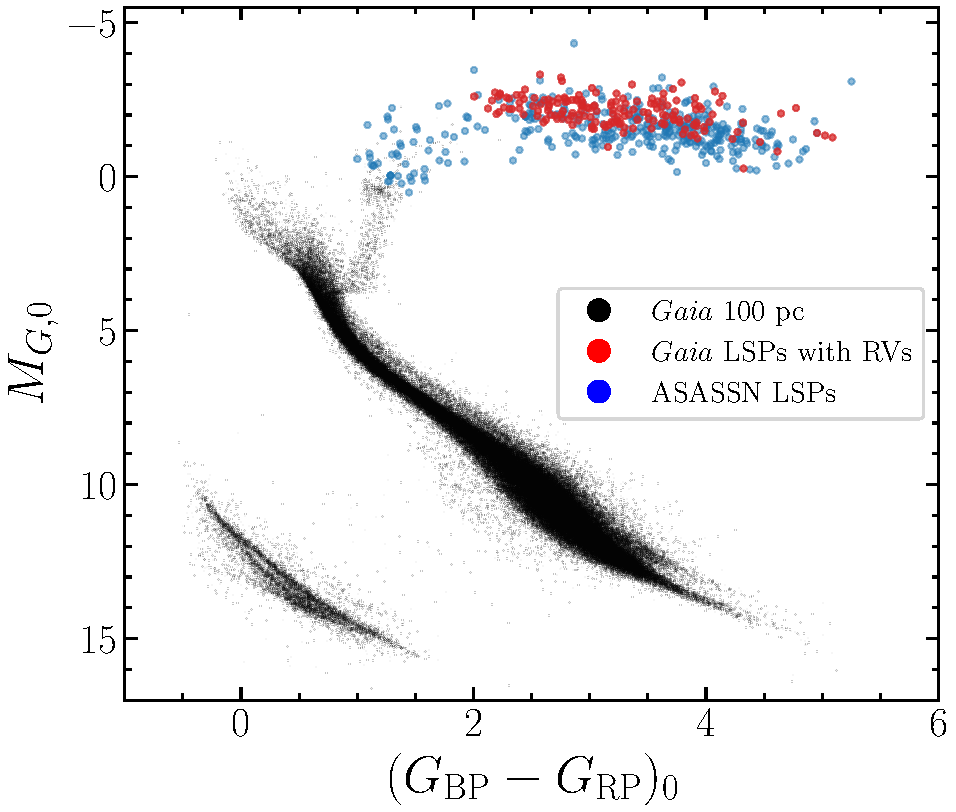
\includegraphics[width=1.0\columnwidth]{Figures/hr_diagram_lsps.pdf}
\caption{Color-magnitude diagram of the LSP samples used in this work. 
We show $1.25$~kpc LSPs from the {\it Gaia} focused product release with RV time-series (red), 
which constitutes the primary sample used in this work, as well as the ASAS--SN LSP sample (blue). 
The cleaned {\it Gaia} 100 pc sample is shown for comparison (black). All {\it Gaia} photometry is dust-corrected.} \label{fig:hr_diagram_lsps}
\end{figure}

These blue ASAS--SN sources trace a lower-luminosity subset of the nearby LSP population. They are fainter in apparent magnitude than the stars in the shared evolved giant-branch region, with median $G=10.49$, compared to $G=9.19$ for the remaining ASAS--SN systems and $G=7.91$ for the {\it Gaia} sample in the same distance range. They also show somewhat shorter LSPs, with median $P_{\rm LSP}\simeq424$~d compared to $566$~d for the redder ASAS--SN systems.

Their absence from the {\it Gaia} sample is best explained by the RV-based selection of the {\it Gaia} FPR. The blue ASAS--SN systems are concentrated toward the low-latitude disk, with $61\%$ at $|b|<10^\circ$ and $39\%$ at $|b|<5^\circ$, compared to $28\%$ and $16\%$ for the {\it Gaia} sample. Within the {\it Gaia} FPR sample, the main CMD trend is a decline in RV signal-to-noise toward fainter systems, while the measured RV amplitudes vary only weakly across the occupied locus. The blue ASAS--SN extension therefore reflects a nearby LSP population that is recovered efficiently in photometry but is underrepresented in the {\it Gaia} RV-selected sample, especially at lower luminosities and low Galactic latitude.


Figure \ref{fig:example_rv_phot} shows an example of the RV and photometric time series observations provided by the {\it Gaia} FPR. The chosen system, Gaia DR3 837969014467045888, exhibits a long secondary period of $711$ days at a distance of $683$~pc. The phase-folded figure reveals a phase offset of $+0.2$ between the RV and photometric time series, consistent with previous results on LSPs \citep[e.g.,][]{Nicholls09,Goldberg24}.
The RV semi-amplitude of $1.48~{\rm km~s^{-1}}$ corresponds to an implied minimum companion mass of $M_2 \sin i=0.08~{\rm M_\odot}$, assuming the RVs are due to orbital motion about a $M_1=1~{\rm M_\odot}$ primary star. These features -- phase offset, period, and RV amplitude -- are broadly similar to the rest of the {\it Gaia} LSP sample (see Appendix \ref{app:all_plots}).

\begin{figure}
\centering
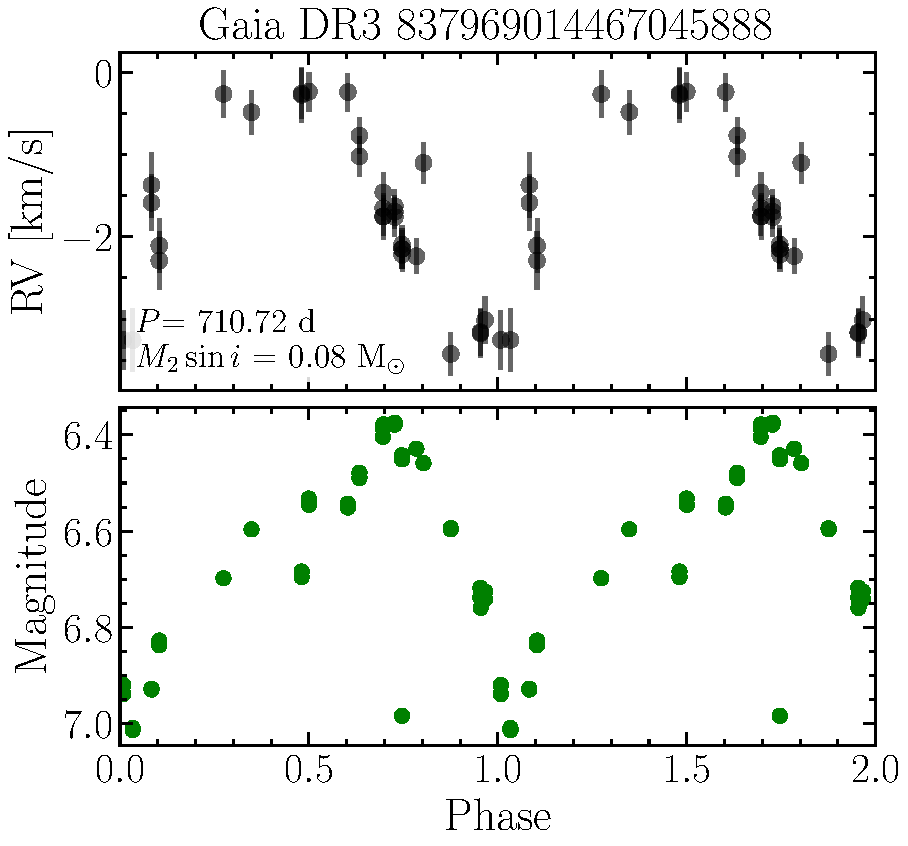
\includegraphics[width=1.0\columnwidth]{Figures/example_rv_phot.pdf}
\caption{Example of RV and photometric time-series observations of LSPs in the {\it Gaia} FPR sample. We show measured RVs (top panel) and $G$-band photometry (bottom panel) for an example LSP: Gaia DR3 837969014467045888. We include both the time series (left) and phase-folded data (right), folded on the long secondary period.
The star resides at a distance of $683$~pc with a long secondary period of $711$~days. If the RV variations were due to orbital motion about a $1~{\rm M_\odot}$ primary, the secondary's minimum mass would be $M_2 \sin i=0.08~{\rm M_\odot}$. For the phase-folded time-series of every {\it Gaia} LSP within $750$~pc, see Appendix \ref{app:all_plots}.
}
\label{fig:example_rv_phot}
\end{figure}



\subsection{Mock {\it Gaia} astrometry}\label{subsec:methodology_gaiamock}

To assess whether the companion masses implied by a binary interpretation of LSPs are compatible with {\it Gaia} astrometric constraints, we generate mock {\it Gaia} observations for each source within $1.5$~kpc (see Section \ref{subsec:methodology_sample}) assuming they are binaries with companion masses derived from RVs. Mock {\it Gaia} observations are simulated for each hypothetical binary using the \texttt{gaiamock} package\footnote{\url{https://github.com/kareemelbadry/gaiamock}} \citep{ElBadry24}. The code simulates epoch astrometric measurements following the {\it Gaia} scanning law and models the effects of orbital motion on the photocenter using the formalism of \citet{Lindegren22}. Measurement uncertainties are assigned using an empirical noise model calibrated on the residuals of well-behaved sources in {\it Gaia} DR3 \citep{Holl23}.

The simulated epoch astrometry is processed through the same cascade of astrometric models employed in the {\it Gaia} DR3 pipeline, including single-star and non-single-star solutions, following the procedures described by \citet{Halbwachs23}. This yields a synthetic astrometric solution for each mock system, including goodness-of-fit statistics that can be directly compared to those reported in the {\it Gaia} DR3 catalog \citep[][]{ElBadry24, ElBadry25}.

A key diagnostic in {\it Gaia} is the re-normalized unit weight error ({\tt RUWE}), which quantifies the quality of the single-star astrometric fit.
By construction, well-modeled single stars have ${\tt RUWE}\approx1$ \citep{Lindegren18}. For unresolved binaries, orbital motion of the photocenter introduces systematic residuals that inflate the {\tt RUWE}, with the magnitude of the effect depending on the orbital parameters, sky position, and apparent magnitude of the system. As a result, {\tt RUWE} provides a sensitive and quantitative diagnostic of unresolved binarity in {\it Gaia} data, and its expected value can be robustly predicted for a given binary configuration using {\tt gaiamock} \citep[e.g.,][]{ElBadry24,ElBadry25}.

In this work, we use an updated version of {\tt gaiamock} designed to improve the reliability of {\tt RUWE} predictions, particularly for systems with small photocenter orbits and for effectively single stars (Iorio et al. 2026, in prep). The default version of the code accurately reproduces the {\tt RUWE} distribution for binaries with clearly detectable astrometric motion \citep[e.g.,][]{ElBadry25}, but systematically underestimates the width of the {\tt RUWE} distribution at low signal-to-noise. The modified version of {\tt gaiamock} used here eliminates CCD-level binning and instead treats individual CCD measurements explicitly. In addition, it applies an empirical, sky-position-dependent rescaling of the epoch-level astrometric uncertainties to reproduce the observed {\tt RUWE} distribution of single stars in {\it Gaia} DR3.


\section{Results}\label{sec:results}

\subsection{RV amplitudes and companion masses}\label{subsec:results_rvamps}

\begin{figure*}
\centering
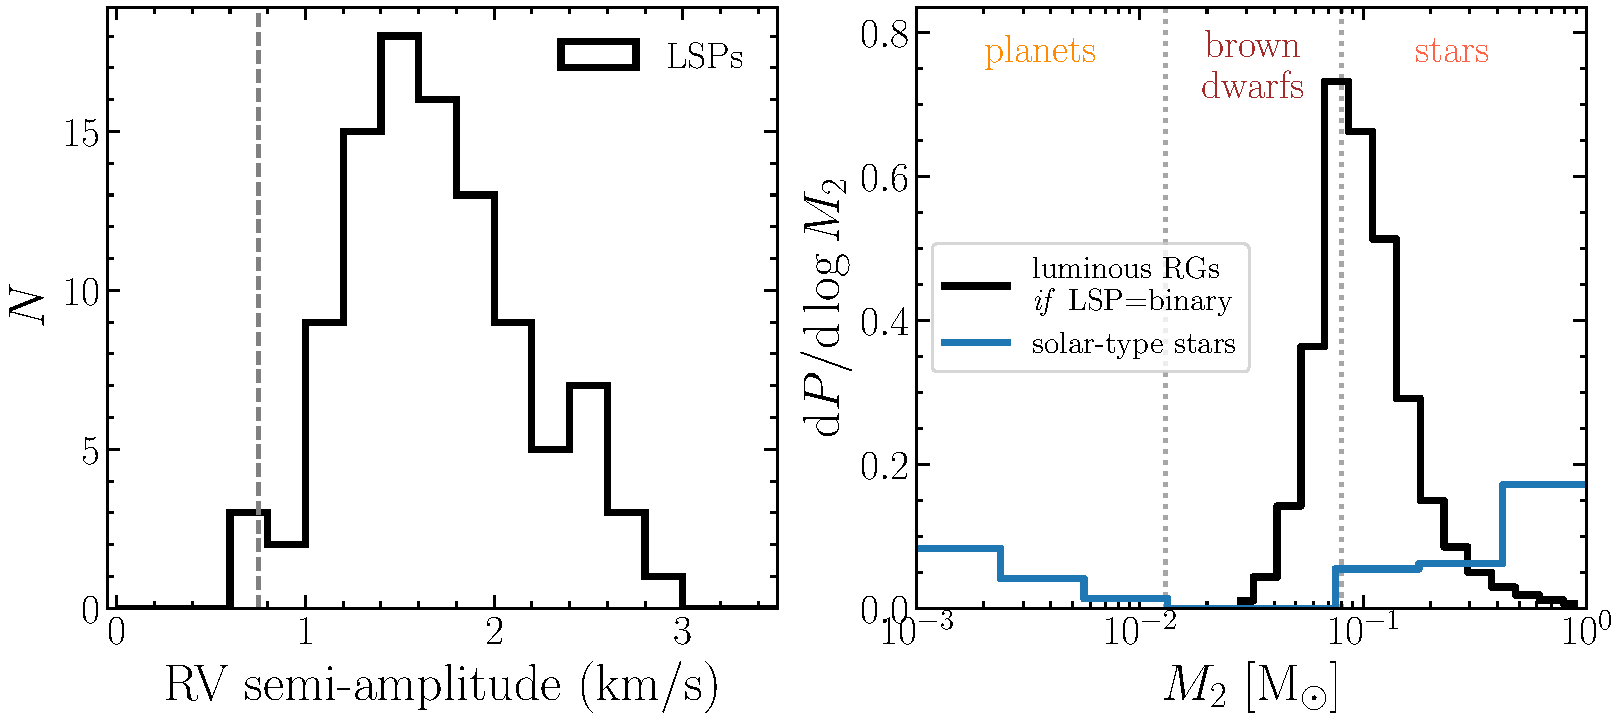
\includegraphics[width=1.0\textwidth]{Figures/rv_amps_m2s.pdf}
\caption{RV semi-amplitude (left) and companion mass (right) distribution of LSPs in the {\it Gaia} $1$~kpc sample ($N=101$). On the left, we show the $K=0.75~{\rm km~s^{-1}}$ line, above which our sample is roughly complete. On the right, the companion mass, $M_2$, is derived from the K assuming a solar-mass primary, circular orbit, and random inclinations. We show the $M_2$ distribution of luminous red giants (solid) and $M_1 \geq 1~{\rm M_\odot}$ solar-type stars \citep{Grether06}. Solar-type stars show a dearth of $0.02-0.1~{\rm M_\odot}$ companions (the ``brown dwarf desert'') whereas luminous red giants ($\sim30\%$ of which are LSPs) suggest ubiquitous $0.02-0.1~{\rm M_\odot}$ companions {\it if} binarity were the cause of LSPs.}
\label{fig:rv_amps_m2s}
\end{figure*}

For each LSP star, we use the observed RV variability to infer the companion mass implied by assuming it is due to Keplerian motion. We adopt a fiducial primary mass of $M_1 = 1~{\rm M_\odot}$ and compute the RV mass function,
\begin{equation}\label{eq:rv_mass_func}
f(M) \equiv \frac{(M_2\sin i)^3}{(M_1+M_2)^2} = \frac{P K^3}{2\pi G}~(1-e^2)^{3/2},
\end{equation}
where $P$ is the LSP period, $K$ is the RV semi-amplitude, $i$ is the orbital inclination, and $e$ is the eccentricity. We assume circular orbits but also test modest eccentricities ($0.1-0.5$), finding that it does not change our conclusions. 


Figure \ref{fig:rv_amps_m2s} shows the distribution of RV semi-amplitudes (left) and the corresponding companion-mass estimates (right) for the $1$~kpc {\it Gaia} LSP sample ($N=101$). The observed RV semi-amplitudes are clustered sharply with median $K  = 1.63~{\rm km~s^{-1}}$ and $~\sigma_K = 0.5~{\rm km~s^{-1}}$. Assuming that the RV variability is due to orbital motion and adopting a fiducial primary mass of $M_1 = 1~{\rm M_\odot}$, these amplitudes translate into a sharply peaked companion-mass ($M_2$) distribution.
The inferred secondary masses peak near the hydrogen-burning limit, with a median $M_2 \sin i = 0.075~{\rm M_\odot}$ ($M_2 \approx 0.09 ~{\rm M_\odot}$) and standard deviation $0.025~{\rm M_\odot}$.


A striking feature of the RV amplitude distribution is the paucity of low-amplitude systems. In the $1$~kpc {\it Gaia} sample, only $5$ out of $101$ stars ($\sim5\%$) have $K<1~{\rm km~s^{-1}}$. Part of this deficit is due to selection effects of the {\it Gaia} FPR sample. In particular, the requirement $\epsilon_{\rm V_R}<0.175\times{\tt rv\_amplitude\_robust}$ implies that the RV semi-amplitude, $K=2\times{\tt rv\_amplitude\_robust}$, must exceed approximately three times the uncertainty on the median RV. For the sample analyzed here, the distribution of median RV uncertainties peaks near $0.25~{\rm km~s^{-1}}$ (standard deviation $0.13~{\rm km~s^{-1}}$), such that systems typically require $K\gtrsim0.7$--$0.8~{\rm km~s^{-1}}$ to be included.

However, selection effects alone cannot explain the observed distribution. Among the $101$ LSP stars, $57$ have $\epsilon_{\rm V_R}<0.25~{\rm km~s^{-1}}$, implying that they are sensitive to RV semi-amplitudes down to $K\approx0.75~{\rm km~s^{-1}}$. Despite being sensitive to low $K$ values, only $5$ of these systems exhibit $K<1~{\rm km~s^{-1}}$. Namely, the RV semi-amplitudes {\it intrinsically} cluster tightly around $K\sim1$--$2~{\rm km~s^{-1}}$, with relatively few systems at $K<1~{\rm km~s^{-1}}$ despite sensitivity there. 

This conclusion is consistent with the independent results of \citet{Nicholls09}, who obtained multi-epoch RV measurements for 58 LSP red giants using the FLAMES/GIRAFFE spectrograph on the VLT \citep{Pasquini02} at a resolving power of $R\approx23{,}900$ over $693.7$--$725.0$~nm. They likewise found a narrow peak in RV semi-amplitudes at $K\approx1.75~{\rm km~s^{-1}}$ and a pronounced deficit of systems below $K\sim1~{\rm km~s^{-1}}$. Through injection--recovery simulations, they demonstrated that their data were sensitive to RV semi-amplitudes below $1~{\rm km~s^{-1}}$, yet detected none, leading them to conclude that the intrinsic RV amplitude distribution of LSP stars is sharply peaked near $K\sim1$--$2~{\rm km~s^{-1}}$. Our results independently confirm this conclusion using the larger sample of {\it Gaia} RVs.

The right panel of Figure \ref{fig:rv_amps_m2s} shows the companion mass distribution of LSPs as inferred from their RV amplitudes, assuming isotropic line-of-sight inclinations and solar mass primaries. We calculate the probability of a luminous red giant (RG), hosting a companion in the $1-3$~au range per logarithmic range of secondary mass ($N_i$) for a bin of width $\Delta \log M_2$ using
\begin{equation}\label{eq:dn_dlogm}
    \frac{{\rm d}P}{{\rm d}\log M_2} = \frac{N_i}{N_{\rm tot}\Delta \log M_2}.
\end{equation}
Because the right-panel LSP curve is normalized per luminous RG rather than per LSP host, its integral is $f_{\rm LSP} \approx 0.3$ \citep[e.g.,][]{Wood99,Wood04,Pawlak21}.
We also calculate this quantity for the $25$~pc sample of solar-type stars with $M_1 \geq 1~{\rm M_\odot}$ \citep[][]{Grether06}, which are the progenitors of luminous RGs. The \citet{Grether06} sample contains $464$ Hipparcos stars, $384$ of which have RVs. They characterize the completeness-corrected distribution of ${\rm d}N/{\rm d}\log M_2 = N_i/\Delta \log M_2$ for companions more massive than Jupiter --  including giant planets, brown dwarfs, and stars -- with orbital periods shorter than $5$~years. Overall, they find that $\sim16\%$ of solar-type primaries have companions in this mass and period range: $\sim5\%$ are giant planets, $\sim11\%$ are stars, and $<1\%$ are brown dwarfs.

The inferred companion-mass distribution for LSP stars is narrow and strongly concentrated near the stellar-substellar boundary (Figure \ref{fig:rv_amps_m2s}). It peaks at $M_2 \approx 0.1~{\rm M_\odot}$, with $36/101$ systems being consistent with brown-dwarf-mass companions ($M_2 < 0.08~{\rm M_\odot}$) and $89/101$ being consistent with companions with $M_2 < 0.15~{\rm M_\odot}$. 

Interpreted as orbital motion, the RV variability of LSPs thereby implies companions with masses of $0.03$-$0.15~{\rm M_\odot}$ with orbits at $\sim1$-$3$~au around evolved solar-type stars (Section~\ref{subsec:results_rvamps}). 
For solar-type stars on the main-sequence, such companions are notoriously rare, defining the ``brown dwarf desert,'' a pronounced deficit of companions with masses $\sim0.02$-$0.2~{\rm M_\odot}$ at separations of a few au around solar-type main-sequence stars \citep[e.g.,][]{Marcy00,Grether06}. This can be appreciated from the $M_2$ distribution of solar-type main-sequence stars shown in Figure \ref{fig:rv_amps_m2s} (blue curve). 
Fewer than $1\%$ of solar-type main-sequence stars have companions in this mass and period range $0.03$-$0.15~{\rm M_\odot}$ whereas $\sim30\%$ of RGs of similar mass show LSPs, about half of which lie in the mass range \citep[][]{Soszynski21,Pawlak24}. Reconciling the high incidence of LSPs ($\sim30\%$) among red giant and AGB stars with the low incidence of brown-dwarf companions orbiting their main-sequence progenitors is a fundamental challenge for binary-based models. 
Furthermore, if such companions exist and survive post-main-sequence evolution, a comparable fraction of white dwarfs should host $\sim0.1~{\rm M_\odot}$ companions at separations of a few au. However, IR excess surveys find brown dwarf companions around $\lesssim1\%$ of white dwarfs \citep[e.g.,][]{Farihi05,Girven11,Steele11}.

One proposed resolution is that many LSP companions did not form at their present masses but were initially planetary-mass companions that grew through wind accretion or mass transfer as the host ascends the giant branch, evolving into brown dwarfs or very low-mass stars \citep[e.g.,][]{Retter05,Soszynski21}. This scenario predicts that LSPs presently reside in binaries with low-mass companions, which would induce astrometric motion to LSPs as observed by {\it Gaia}. We test this prediction in Section \ref{subsec:results_ruwe}.

\subsection{Gaia {\tt RUWE}}\label{subsec:results_ruwe}
To test the binary interpretation of LSPs, we compare the astrometric signal predicted from the RV-inferred orbits to the observed {\it Gaia} astrometry. Assuming that the RV variability is from a companion's orbit, we forward-model the corresponding {\it Gaia} DR3 astrometric observations and compare them to the observed {\tt RUWE} values.

We forward-model the {\it Gaia} astrometric response expected for these hypothetical binaries using {\tt gaiamock} \citep{ElBadry24}. For each star, we construct a binary model with period fixed to the observed LSP, minimum companion mass ($M_2 \sin i$) fixed to the RV-inferred value, and primary mass fixed to $1~{\rm M_\odot}$. We assume a dark companion that contributes negligible flux compared to the evolved star, such that the photocenter follows the primary to excellent approximation\footnote{In the optical {\it Gaia} G band, a $1~{\rm M_\odot}$ red giant at LSP luminosities typically provides $\sim10,000$ times more flux than the highest-mass M dwarf; we therefore neglect secondary light when computing the photocenter orbit for these typical M-dwarf or brown dwarf companions.}. We sample orbital inclinations isotropically (uniform in $\cos i$) and draw the longitude of the ascending node $\Omega$ and argument of periastron $\omega$ from uniform distributions $\mathcal{U}(0,2\pi)$. For each star we generate $50$ Monte Carlo realizations, each time (a) drawing angles, (b) running {\tt gaiamock} to produce synthetic epoch astrometry at the star's sky position and brightness, and (c) recording the resulting {\tt RUWE} from the best-fit single-star solution. Our fiducial models assume $e=0$, however, since tides can be weaker for low-mass companions \citep{Zahn77} and eccentric LSP-companion orbits have been proposed previously \citep[e.g.,][]{Decin25}, we repeat the analysis with $e=0.3$ and find that it does not change our conclusions. For each star, we compare the observed {\tt RUWE} from {\it Gaia} DR3 to the distribution of {\tt RUWE} values predicted across Monte Carlo realizations, thereby testing whether the RV-inferred companions are compatible with {\it Gaia} data.

\begin{figure}
\centering
\includegraphics[width=1.0\columnwidth]{Figures/RUWE_all.pdf}
\caption{Observed vs predicted {\tt RUWE} for LSP stars assuming the binary hypothesis. 
The left panel shows the observed {\it Gaia} {\tt RUWE} while the right panel shows the predicted {\tt RUWE} assuming the RV variability is due to a binary companion. We display results for three different samples, restricted to $1.5$~kpc: {\it Gaia} LSPs (top), ASAS--SN LSPs (middle), and {\it Gaia} ellipsoidal variables (ELL; bottom). Note that the ASAS--SN sample does not have RVs. The red dashed line shows ${\tt RUWE}=1$. 
The nearest LSPs are predicted to show inflated {\tt RUWE} values if the LSP was due to binarity, however, they do not. In contrast, the nearest ellipsoidal variables are predicted to show inflated {\tt RUWE} values if the RV variability is due to binarity, which they do.
}
\label{fig:RUWE}
\end{figure}


Figure \ref{fig:RUWE} compares the {\tt RUWE} values predicted under the binary hypothesis to those measured in {\it Gaia} DR3. The left column shows the observed {\tt RUWE} as a function of distance from {\it Gaia} DR3 while the right column shows predictions assuming LSPs reside in binaries. The error bars reflect $1\sigma$ uncertainties ($16$th-$84$th percentile).
We show the results for three samples: (1) {\it Gaia} LSPs, (2) ASAS--SN LSPs, and (3) {\it Gaia} ellipsoidal variables (ELL), also selected from the Gaia LPV sample of \citep[][]{Gaia_FPR}. The {\it Gaia} ELL sample serves as a control to demonstrate that {\tt RUWE} closely tracks binarity, particularly in the nearest systems ($d\lsim1.5$~kpc).

If the LSPs were due to orbiting companions with masses implied by their RVs (often $\approx0.1~{\rm M_\odot}$; see Figure \ref{fig:rv_amps_m2s}) the binary motion would be detected by {\it Gaia} and lead to inflated {\tt RUWE} values for the closest systems (top two panels). However, this is not observed. Instead, the majority of LSPs within $750$~pc ($80\%$, $58/73$) show predicted {\tt RUWE} larger than observed, indicating that the astrometric motion expected from the companion is not present in the {\it Gaia} data. A small number of systems do show elevated {\tt RUWE} values consistent with unresolved binaries. However, these objects do not show the strong increase in {\tt RUWE} toward smaller distances predicted if the majority of LSPs were binaries (top-right panel), indicating that such cases represent a minority of the population.
The discrepancy between observed and predicted {\tt RUWE} persists out to $d\lesssim750$~pc, where the astrometric reflex from $0.1~{\rm M_\odot}$ companions is detectable in {\it Gaia} DR3. 
In contrast, the {\it Gaia} ellipsoidal variable candidates, which typically have $K\approx10~{\rm km~s^{-1}}$ ($M_2\approx0.65~{\rm M_\odot}$), show observed values of ${\tt RUWE}>1$. Indeed, our {\tt gaiamock} forward model using their RV amplitudes predicts relatively large {\tt RUWE} values, consistent with {\it Gaia} observations and with them being genuine binaries.

In short, if LSPs were caused by binary companions with masses inferred from their RV amplitudes ($0.03-0.2~{\rm M_\odot}$), the resulting orbital motion should produce detectable astrometric signatures and inflate the {\it Gaia} {\tt RUWE} of nearby systems. Instead, we find that the observed {\tt RUWE} of LSPs under the binary hypothesis is significantly smaller than the predicted value, indicating that the expected astrometric reflex motion is not present. By contrast, known ellipsoidal-variable binaries show elevated {\tt RUWE} values in {\it Gaia}, which are consistent with what is predicted from their RV amplitudes with the forward model (Figure \ref{fig:RUWE}). We therefore conclude that (sub)stellar companions with masses implied by the RV variability are not the dominant cause of long secondary periods in red giants.

\section{Discussion}\label{sec:discussion}

\subsection{Implications for binary models}\label{subsec:implications_for_binarity}

Binary companions have long been considered one of the leading explanations for long secondary periods. In these models, the LSP is identified with the orbital period of a low-mass stellar or substellar companion, while the photometric variability is attributed to periodic obscuration by dust, modulation of circumstellar material near the companion, or tidally induced variability \citep[e.g.,][]{Wood99,Wood04,Soszynski07,Soszynski14,Soszynski21,Percy23,Goldberg24,Decin25}. 

Interpreting the observed RV variations as orbital motion implies companions with masses clustered near the stellar--substellar boundary (Figure \ref{fig:rv_amps_m2s}) on au-scale orbits (Section~\ref{subsec:results_rvamps}), in the same region as the brown dwarf desert around solar-type stars, the progenitors of most LSPs.
Reconciling this demographic with the high incidence of LSPs ($\sim30\%$) among evolved red giants has long posed a challenge for binary-based LSP models. A proposed reconciliation is that many LSP companions were initially massive planets that accreted material up to their present mass \citep[e.g.,][]{Retter05,Soszynski21}. 

Irrespective of the hypothetical companion's origin, all companion-based LSP models share a fundamental and testable prediction: a companion massive enough to generate the observed RV amplitudes (a few ${\rm km~s^{-1}}$) is present today. Our results show that such companions {\it should} induce {\it Gaia}-detectable astrometric reflex motion of the red giant, and that such motion is absent in {\it Gaia} observations. 
This prediction is largely independent of the specific mechanism producing the photometric variability, or the origin of the companion.
This conclusion is also robust to orbital configuration and applies to models invoking eccentric orbits or indirect modulation of circumstellar dust, since the dust contributes negligibly to the optical photocenter measured by \textit{Gaia}.

One potential concern is that intrinsic stellar variability could also induce astrometric jitter, possibly elevating {\tt RUWE}. 
Three-dimensional radiative-hydrodynamic simulations of red supergiants predict that large convective cells can shift the stellar photocenter by $\sim1$--$5\%$ of the stellar radius, potentially contributing to {\it Gaia} astrometric errors \citep{Chiavassa22}. 
However, a detailed analysis of {\it Gaia} astrometry shows that such photocenter motions are presently undetectable: the measured excess astrometric noise in {\it Gaia} DR3 is dominated by other noise sources and is typically an order of magnitude larger than the predicted convective signal \citep{Kochanek23}. 
The absence of elevated {\tt RUWE} in LSP stars therefore does not conflict with models invoking convection or radial pulsations, although it may still disfavor variability mechanisms that produce large non-axisymmetric surface brightness structures capable of generating detectable photocenter shifts.

Taken together, our findings rule out low-mass stellar and substellar companions as the {\it dominant} cause of LSPs in giant branch stars. 
While binarity may still influence the circumstellar environment in individual systems, companion-induced orbital motion cannot account for the LSP phenomenon as a population-wide explanation, motivating renewed focus on alternative stellar mechanisms, possibly intrinsic to the star, as the origin of LSPs.

\subsection{Betelgeuse }\label{subsec:betelgeuse}

$\alpha$~Orionis (Betelgeuse), the tenth brightest star in the sky and the nearest red supergiant \citep{Hoffleit82}, is frequently discussed as an LSP system. 
Although Betelgeuse is more massive and luminous than the RGB and AGB stars that dominate our sample, it is nonetheless considered an LSP star: it shows variability on timescales of $\sim400$~days, commonly attributed to pulsation, and $\sim2100$~days, widely identified as its LSP \citep[e.g.,][]{Joyce20}. 
Betelgeuse's LSP behavior, both in photometry and RVs, is broadly similar to those of lower-mass LSP variables, making it a natural benchmark for proposed binary models.


Recent studies have interpreted Betelgeuse’s LSP as evidence for a low-mass companion \citep{Goldberg24,MacLeod25}. 
Using century-long RV and astrometric data, \citet{MacLeod25} propose a companion of mass $\lesssim1~{\rm M_\odot}$ on a $\sim2110$~day orbit at a separation of $\sim2$--$3\times$ Betelgeuse’s radius. 
Although this companion mass is larger than the $\sim0.1~{\rm M_\odot}$ companions implied for typical LSP stars in our sample, the inferred mass ratio ($M_2/M_1 \sim 0.05$--$0.1$) and measured RV semi-amplitude ($K \approx 1.5 \pm 0.34~{\rm km~s^{-1}}$) lies squarely at the peak of the LSP RV amplitude distribution (Figure \ref{fig:rv_amps_m2s}).
Their model invokes tidal spin--orbit coupling and a dust-rich wake trailing the companion to explain Betelgeuse’s anomalously rapid rotation and photometric phase offset, similar to earlier interpretations based on circumstellar dust modulation \citep[e.g.,][]{Goldberg24}. However, as \citet{MacLeod25} discuss, the astrometric signal could also be modeled as large-amplitude white noise, and that more data will be needed to test the binary interpretation. \citet{Goldberg24} measure similar companion properties of $1.17 \pm 0.07~{\rm M_\odot}$ at a radius of  $2.43^{+0.21}_{-0.32}$ times the radius of Betelgeuse. Antares, another one of the closest red supergiants \citep[$d=170$~pc][]{vanLeeuwen07}, also shows an LSP ($P \simeq 2167$~days) with an RV semi-amplitude of $2.73~{\rm km~s^{-1}}$, implying a low-mass companion ($M_2 \sin i/M_1 \approx 0.07$) if interpreted as orbital motion \citep{Pugh13}.

Most recently, optical speckle observations of Betelgeuse obtained near the predicted quadrature reported a probable point source at the expected separation ($\approx52$~mas) and position angle, although at alarmingly low significance ($\sim1.5\sigma$; \citealt{Howell25}). 
Additional spectroscopic work has interpreted time-variable absorption and outflow signatures as evidence for a companion-induced wake within the extended atmosphere of the star \citep{Dupree26}.

Recent direct searches have also placed constraints on the proposed companion. 
Deep {\it Chandra} observations obtained near the predicted orbital quadrature detected no X-ray source at the position of Betelgeuse, implying an upper limit of $L_X \lesssim 2\times10^{30}$ erg s$^{-1}$ and ruling out an accreting compact object such as a white dwarf or neutron star \citep{OGrady25}. 
Complementary far-UV spectroscopy with {\it HST}/STIS likewise detected no spectral features at the predicted velocity of the companion and excludes companions with masses $\gtrsim1.5\,M_\odot$ or FUV emission exceeding $\sim10^{-14}$ erg s$^{-1}$ cm$^{-2}$ \AA$^{-1}$ in the $1200$--$1700$ \AA\ band \citep{Goldberg25}. 
These observations therefore rule out several classes of luminous or accreting companions but remain consistent with a faint low-mass young stellar object.

Alternative interpretations attribute Betelgeuse’s long period to intrinsic stellar variability. Non-adiabatic pulsation models suggest that the $\sim2100$~day signal may correspond to the fundamental radial mode of the star rather than to orbital motion \citep{Saio23}. 

Our results provide a population-level test of the binary interpretation for LSPs, which {\it disfavors} low-mass companions as the dominant cause of LSPs in evolved giants. Given that Betelgeuse’s RV amplitude, photometric amplitude, period, and implied mass ratio are typical of the LSP population, it seems plausible that its LSP may likewise arise from an alternative stellar variability mechanism rather than from orbital motion from a binary companion. 

However, since our results focus on the LSP population as a whole, and not Betelgeuse in particular, it remains possible that Betelgeuse represents a special or borderline case where binarity does cause the LSP.
Continued monitoring, particularly near future orbital quadratures, will therefore be crucial for determining whether Betelgeuse's LSP is an exceptional case of binarity or whether its variability reflects the same physical processes operating in the broader LSP population.


\section{Conclusions}\label{sec:conclusions}

More than a century after their discovery, the origin of long secondary periods (LSPs) remains unknown, despite being observed in $\sim1/3$ of pulsating luminous RGB and AGB stars. 
Low-mass stellar or substellar companions have emerged as one of the leading explanations for LSPs, particularly in recent years \citep[e.g.,][]{Soszynski21,Goldberg24,MacLeod25,Decin25}. In these models, the LSP corresponds to a companion's orbital period, while the photometric variability is attributed to occultation or modulation of circumstellar material. In this work, we provide a direct, population-wide test of the binary LSP hypothesis using a combination of RVs, photometry, and astrometry available from the {\it Gaia} Focused Product Release \citep{Gaia_FPR}.

Using RVs for a sample of nearby LSP stars (e.g., Figure \ref{fig:example_rv_phot}), we infer the companion masses ($M_2$) implied under the binary hypothesis. The observed RV semi-amplitudes cluster sharply around $K\approx1.6~{\rm km~s^{-1}}$, corresponding to inferred companion masses narrowly peaked near $M_2\approx0.09~{\rm M_\odot}$ (Figure \ref{fig:rv_amps_m2s}). We then forward-model the expected astrometric signatures of these hypothetical companions using {\tt gaiamock} \citep{ElBadry24} and compare them to the observed {\it Gaia} astrometry. We find that the predicted re-normalized unit weight error ({\tt RUWE}) values are systematically larger than those observed (Figure \ref{fig:RUWE}). Namely, for $80\%$ of the local sample, the expected astrometric signal from binarity is {\it not} present in observations. In contrast, known ellipsoidal variable binaries show the elevated {\tt RUWE} in {\it Gaia} that is consistent with the {\tt RUWE} predicted from their RV amplitudes. 

We conclude that low-mass stellar or substellar companions are {\it not} the dominant cause of LSPs in evolved giant branch stars. This conclusion is robust to all such companions, irrespective of their specific variability-causing mechanism, orbital configuration, or origin. For example, it applies equally to models invoking eccentric orbits or indirect modulation of circumstellar dust, which does not significantly affect the optical photocenter measured by {\it Gaia}. While binarity may influence the circumstellar environment in individual systems, companion-induced orbital motion cannot explain the LSP phenomenon as a population-wide mechanism.

Some of the nearest and brightest red supergiants, such as Betelgeuse, show long-term variability attributed to LSPs \citep[e.g.,][]{Kiss06,Joyce20,Goldberg24, MacLeod25}.
Given that Betelgeuse shows an RV amplitude, photometric amplitude, period, and implied mass ratio typical of the broader LSP population \citep[e.g.,][]{Goldberg24,MacLeod25}, our results suggest that its LSP may likewise arise from an alternative physical mechanism rather than from orbital motion from a binary companion, although it may represent a special case.

Looking ahead, the empirical constraints established by the {\it Gaia} sample and many previous works provide an extensive list of LSP properties -- such as RV amplitudes, phase offsets between RV and photometric variability, and IR behavior -- that successful LSP models should reproduce. These results motivate a renewed focus on stellar mechanisms that do not require a low-mass companion as the driver of LSPs, such as non-adiabatic pulsation, oscillatory convective modes, or the coupling between pulsation, convection, and dust formation in extended giant atmospheres. 


\section{Acknowledgments} \label{acknowledgments}
C.S. acknowledges support from the Department of Energy Computational Science Graduate Fellowship.
This material is based upon work supported by the U.S. Department of Energy, Office of Science, Office of Advanced Scientific Computing Research, under Award Number DE-SC0026073. 

\appendix 
\section{All RV and Photometric time series}\label{app:all_plots}
In Figures \ref{fig:all_phases_1} and \ref{fig:all_phases_2} we show the phase-folded RV and light curves for all targets in the $750$~pc sample.

\begin{figure}
\centering
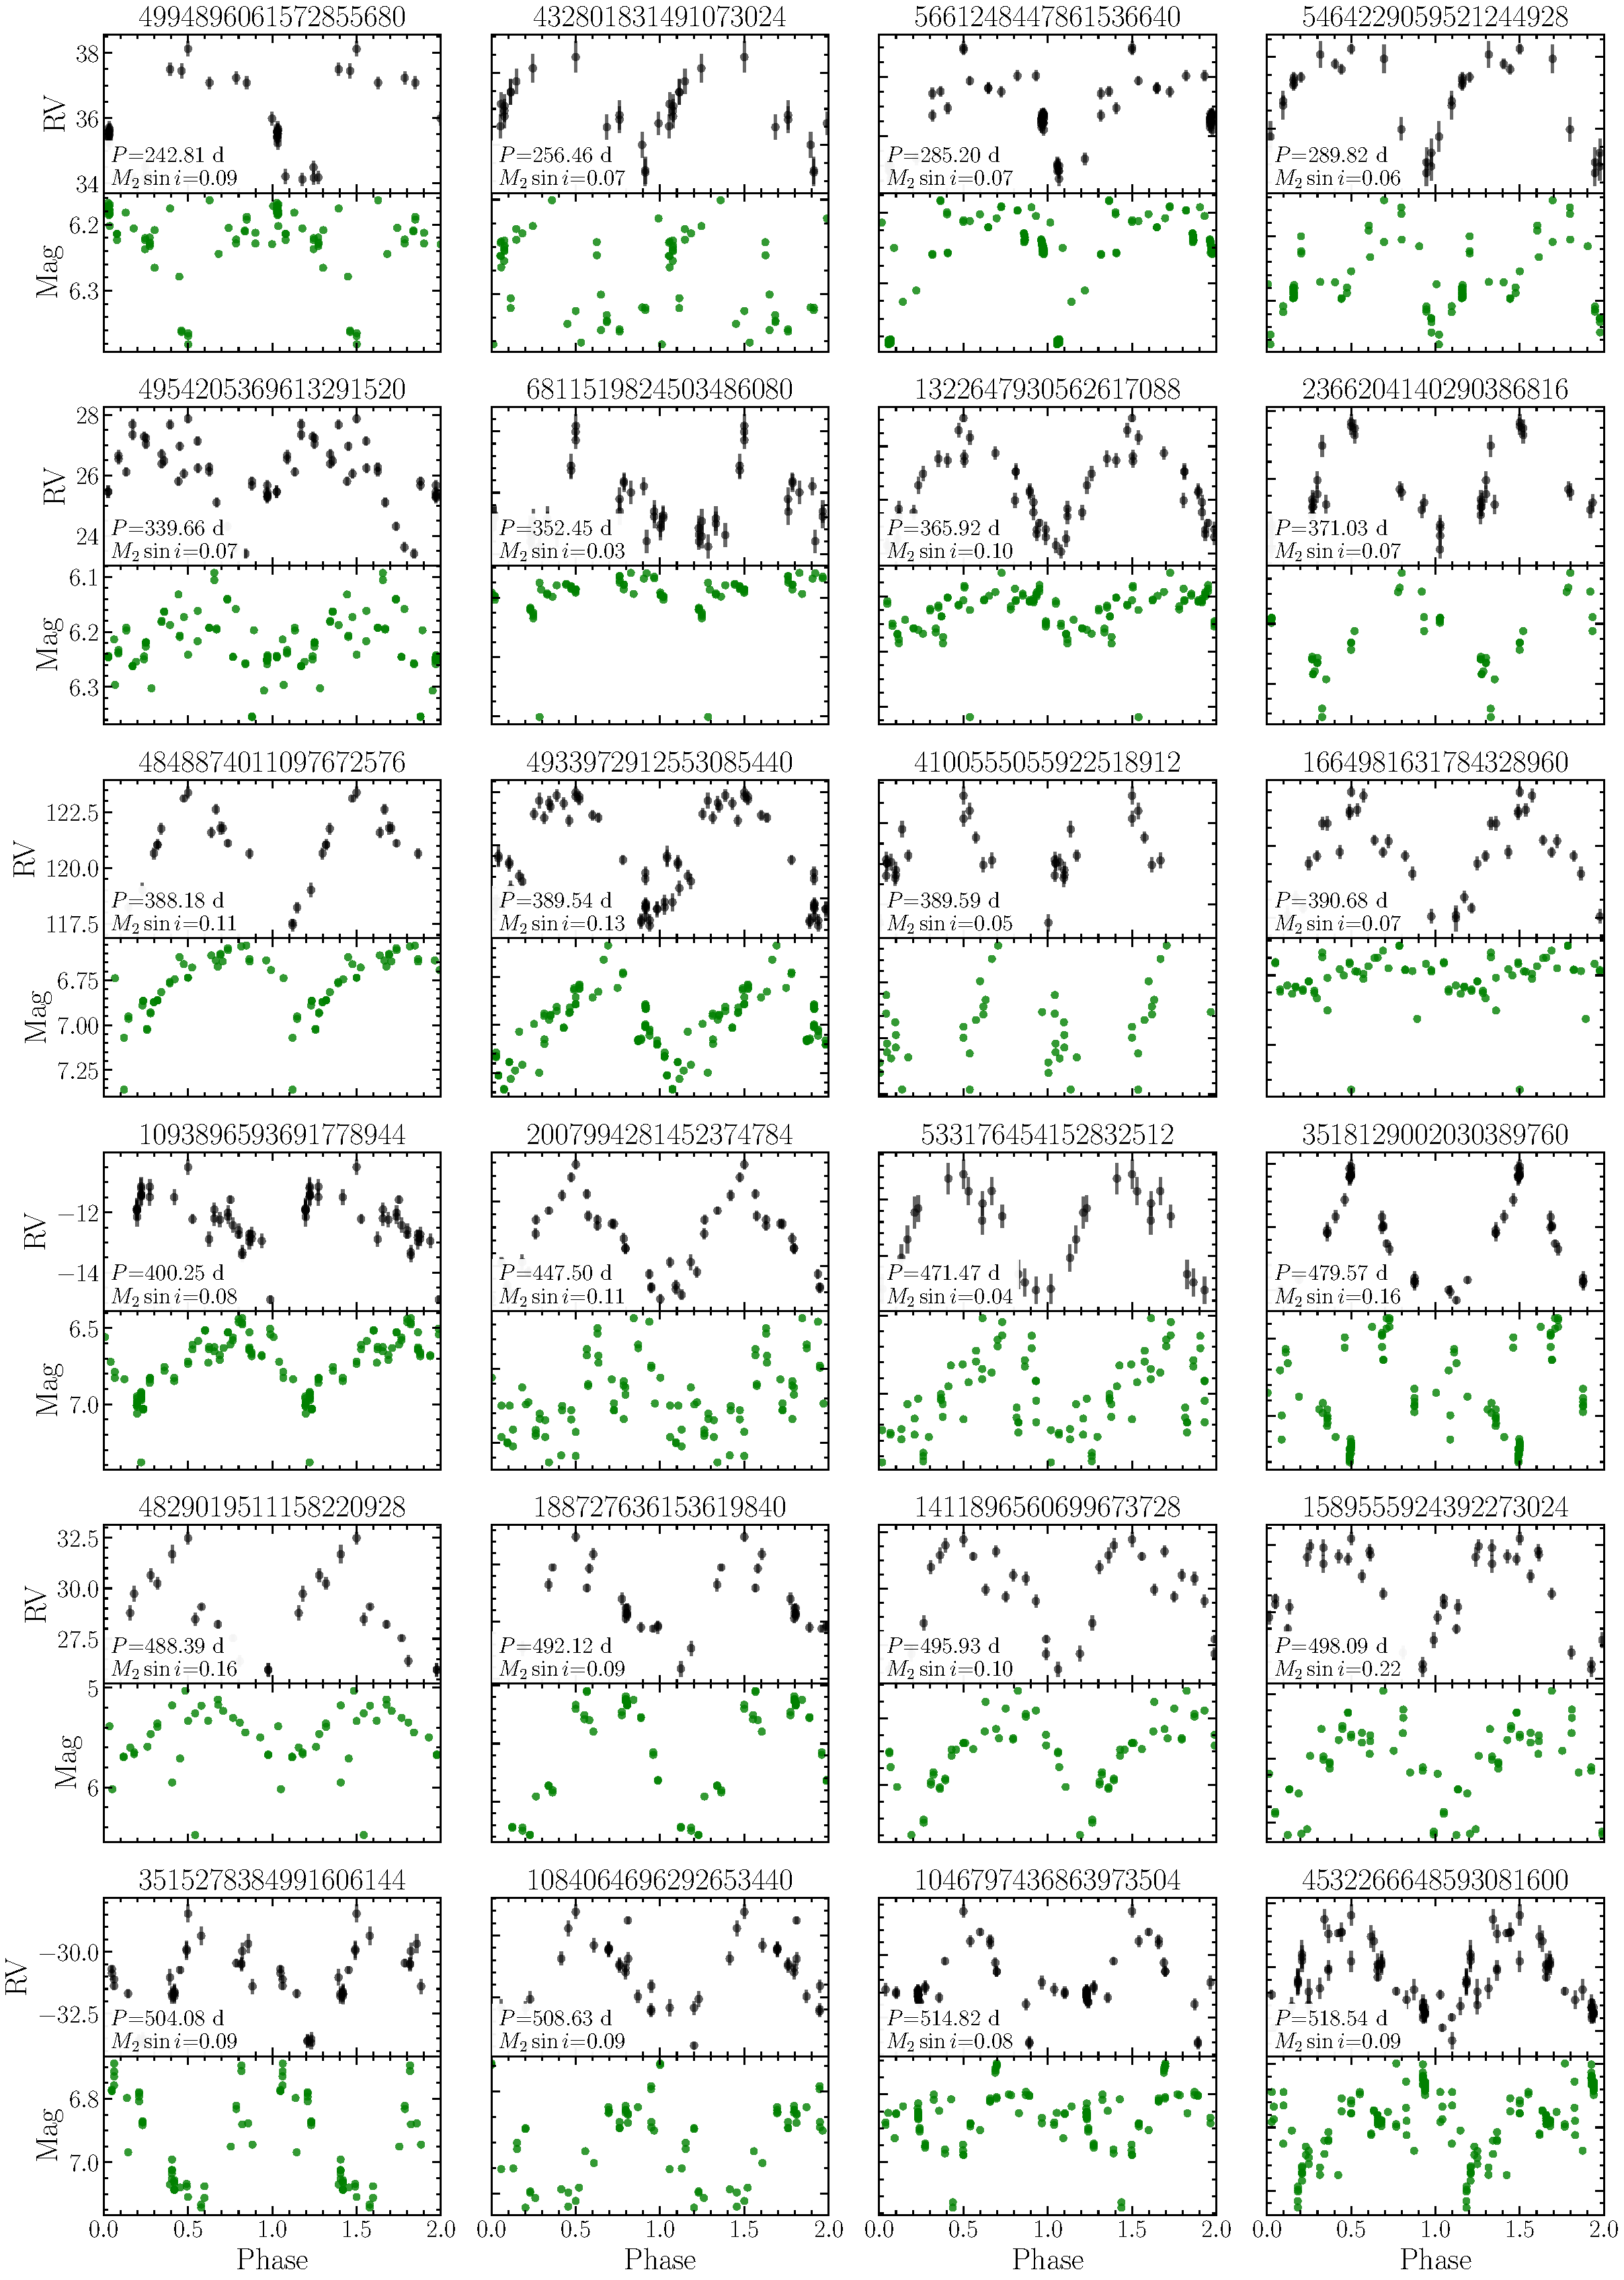
\includegraphics[width=0.8\columnwidth]{Figures/all_phaseplots_grouped_part1.pdf}
\caption{Phase-folded RV and light curves for all {\it Gaia} LSPs within $750$~pc.
}
\label{fig:all_phases_1}
\end{figure}

\begin{figure}
\centering
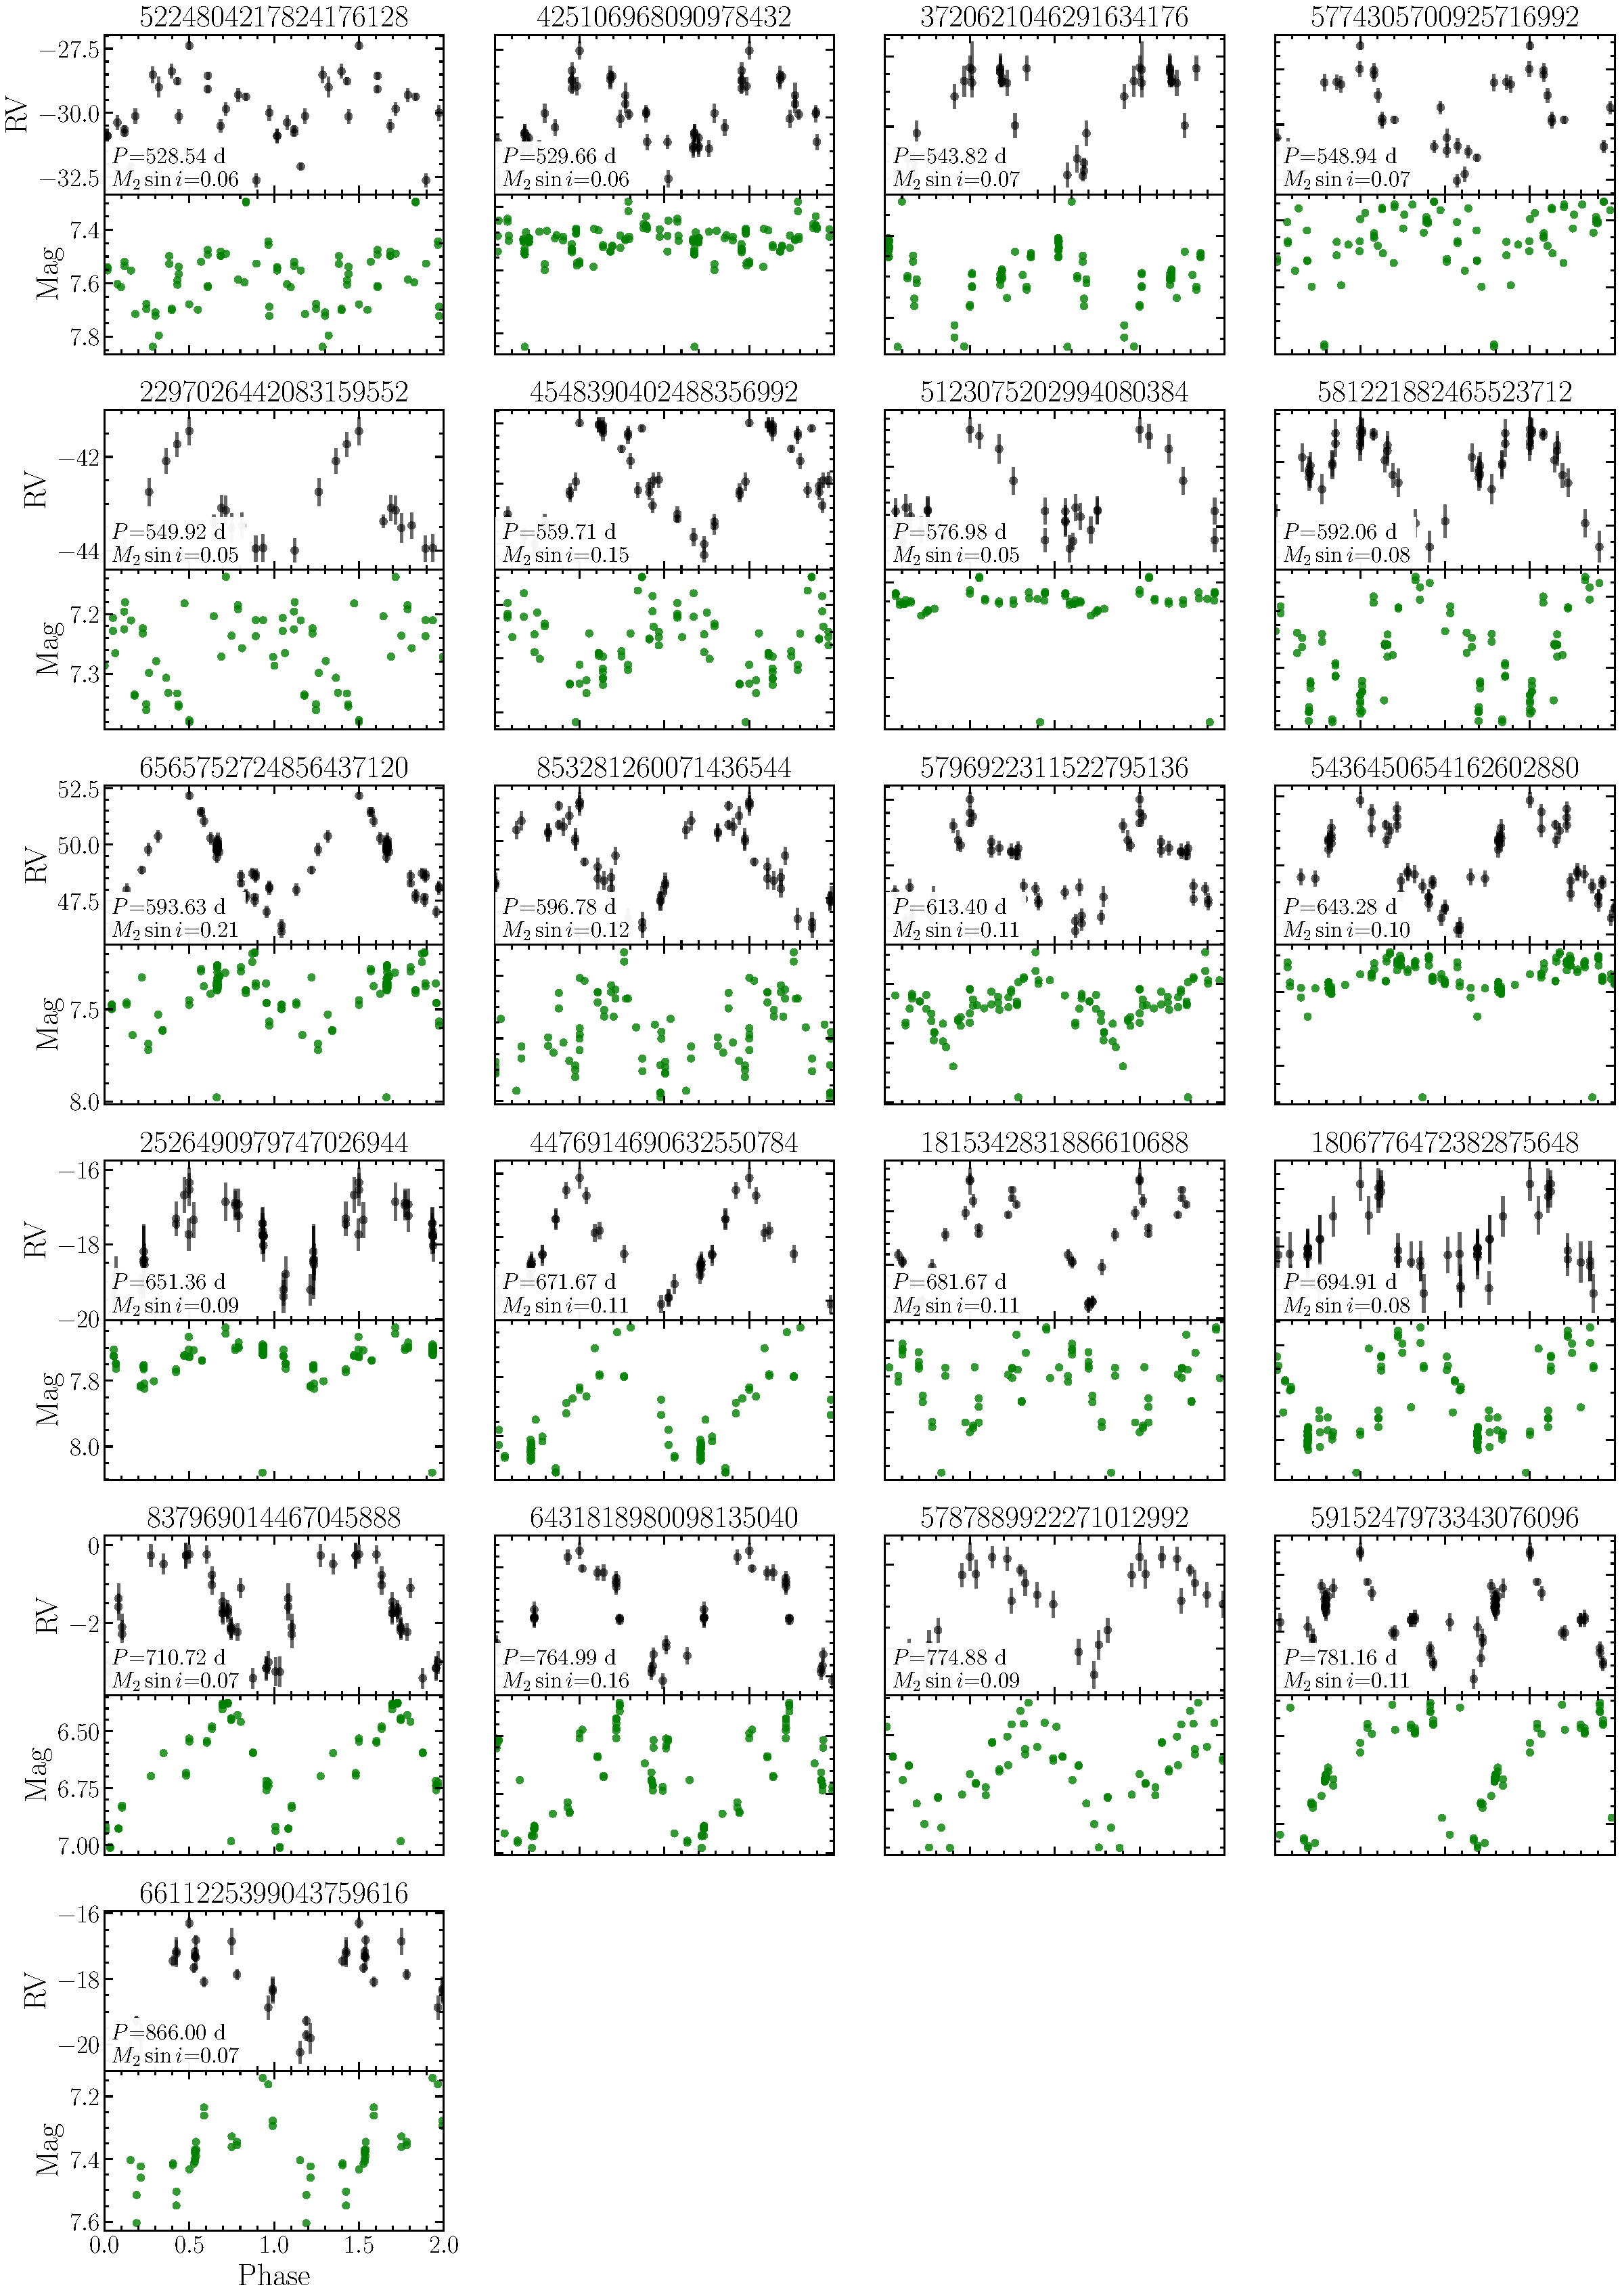
\includegraphics[width=0.8\columnwidth]{Figures/all_phaseplots_grouped_part2.pdf}
\caption{{\bf Continuation of Figure \ref{fig:all_phases_1}.}
}
\label{fig:all_phases_2}
\end{figure}

\clearpage
\bibliography{references}

\end{document}


